\pdfminorversion=4
\documentclass[aspectratio=169]{beamer}

\mode<presentation>
{
  \usetheme{default}
  \usecolortheme{default}
  \usefonttheme{default}
  \setbeamertemplate{navigation symbols}{}
  \setbeamertemplate{caption}[numbered]
  \setbeamertemplate{footline}[frame number]  % or "page number"
  \setbeamercolor{frametitle}{fg=white}
  \setbeamercolor{footline}{fg=black}
} 

\usepackage[english]{babel}
\usepackage{inputenc}
\usepackage{tikz}
\usepackage{courier}
\usepackage{array}
\usepackage{bold-extra}
\usepackage{minted}
\usepackage[thicklines]{cancel}
\usepackage{fancyvrb}

\xdefinecolor{dianablue}{rgb}{0.18,0.24,0.31}
\xdefinecolor{darkblue}{rgb}{0.1,0.1,0.7}
\xdefinecolor{darkgreen}{rgb}{0,0.5,0}
\xdefinecolor{darkgrey}{rgb}{0.35,0.35,0.35}
\xdefinecolor{darkorange}{rgb}{0.8,0.5,0}
\xdefinecolor{darkred}{rgb}{0.7,0,0}
\definecolor{darkgreen}{rgb}{0,0.6,0}
\definecolor{mauve}{rgb}{0.58,0,0.82}

\title[2023-05-09-chep23-analysis-of-physicists]{Analysis of physics analysis}
\author{Jim Pivarski}
\institute{Princeton University -- IRIS-HEP}
\date{May 9, 2023}

\usetikzlibrary{shapes.callouts}

%% Thanks to https://github.com/gpoore/minted/issues/288
\makeatletter
%
% Similar to \EscVerb.
%
% \EscMintinline[options]{<language>}{<backslash-escaped text>}
%
\def\EscMintinline{%
  \FVExtraRobustCommand
  \RobustEscMintinline
  \FVExtraUnexpandedReadOArgMArgEscVArg}

\NewExpandableDocumentCommand \FVExtraUnexpandedReadOArgMArgEscVArg { o m m } {%
  \IfNoValueTF{#1}
    {\FVExtraAlwaysUnexpanded
      {\FVExtraUnexpandedReadOArgMArgEscVArg{#2}{#3}}}
    {\FVExtraAlwaysUnexpanded
      {\FVExtraUnexpandedReadOArgMArgEscVArg[#1]{#2}{#3}}}%
}

\newrobustcmd\RobustEscMintinline[2][]{%
  % similar to \mintinline
  \begingroup
  \setboolean{minted@isinline}{true}%
  \minted@configlang{#2}%
  \setkeys{minted@opt@cmd}{#1}%
  \minted@fvset
  \begingroup
  \@ifnextchar\bgroup
    {\FVExtraDetokenizeREscVArg{\minted@inline@iii}}%
    {\PackageError{minted}%
     {\string\EscMintinline\space delimiters must be paired curly braces in this context}%
     {Delimit argument with curly braces}}}
\makeatother

\begin{document}

\logo{\pgfputat{\pgfxy(0.11, 7.4)}{\pgfbox[right,base]{\tikz{\filldraw[fill=dianablue, draw=none] (0 cm, 0 cm) rectangle (50 cm, 1 cm);}\mbox{\hspace{-8 cm}
\includegraphics[height=1 cm]{princeton-logo-long.png}\hspace{0.1 cm}\raisebox{0.1 cm}{
\includegraphics[height=0.8 cm]{iris-hep-logo-long.png}}\hspace{0.1 cm}}}}}

\begin{frame}
  \titlepage
\end{frame}

\logo{\pgfputat{\pgfxy(0.11, 7.4)}{\pgfbox[right,base]{\tikz{\filldraw[fill=dianablue, draw=none] (0 cm, 0 cm) rectangle (50 cm, 1 cm);}\mbox{\hspace{-8 cm}
\includegraphics[height=1 cm]{princeton-logo.png}\hspace{0.1 cm}\raisebox{0.1 cm}{
\includegraphics[height=0.8 cm]{iris-hep-logo.png}}\hspace{0.1 cm}}}}}

% Uncomment these lines for an automatically generated outline.
%\begin{frame}{Outline}
%  \tableofcontents
%\end{frame}

%% https://indico.jlab.org/event/459/contributions/11547/

%% Analysis of physics analysis
%%  9 May 2023, 16:00
%%  15m
%%  Marriott Ballroom VI-VII (Norfolk Waterside Marriott)

%% Speaker
%%  Pivarski, Jim (Princeton University)
%% Description
%% Data analysis in particle physics is socially distributed: unlike centrally developed and executed reconstruction pipelines, the analysis work performed after Analysis Object Descriptions (AODs) are made and before the final paper review—which includes particle and event selection, systematic error handling, decay chain reconstruction, histogram aggregation, fitting, statistical models, and machine learning—are often performed “off the GRID.”

%% This presents a challenge for developers of analysis tools, who need to know how their tools are being used in order to focus efforts in development, documentation, and training. The most common methods have traditionally been direct conversations with known users, wide-cast surveys, and download counts, but each of these has its limitations.

%% In this talk, I will discuss the above as well as new methods of analyzing user behavior: collecting issue comments through GitHub and GitLab APIs, statically analyzing code from thousands of git repositories matching search criteria, and web analytics of documentation sites. Applying these methods to the Awkward Array library reveals the most commonly used functions, slice idioms, and data types, as well as what libraries Awkward Array is commonly used with and how data are transferred between them. Finally, I apply these methods to other physics analysis libraries to show the generality of the techniques.

%% Consider for long presentation	No

% START START START START START START START START START START START START START

\begin{frame}{Dark computing}
\vspace{0.25 cm}
\begin{columns}
\column{1.1\linewidth}
\only<1>{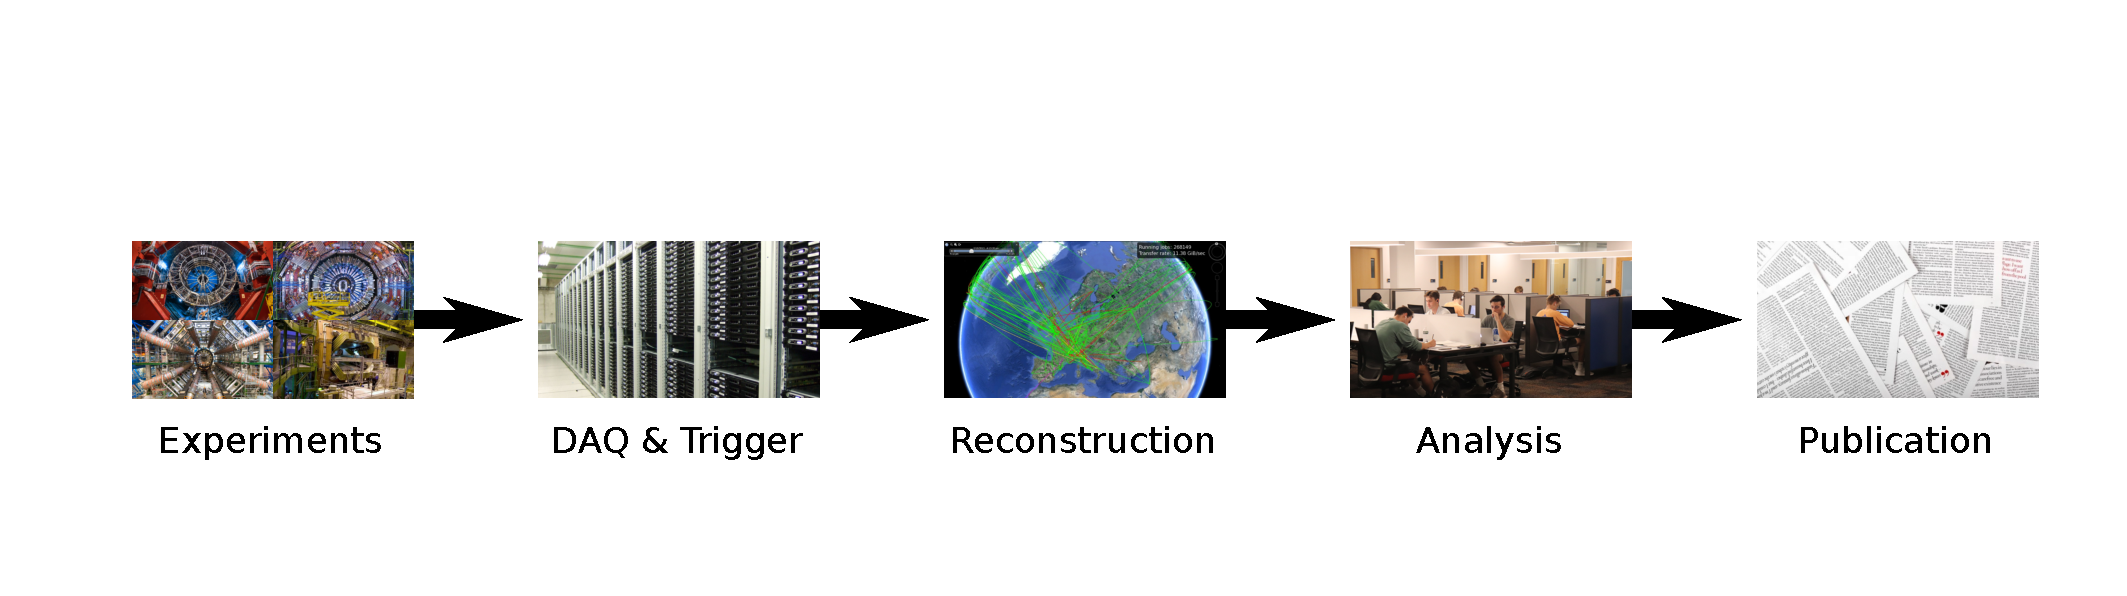
\includegraphics[width=\linewidth]{PLOTS/analysis-chain-0.pdf}}\only<2->{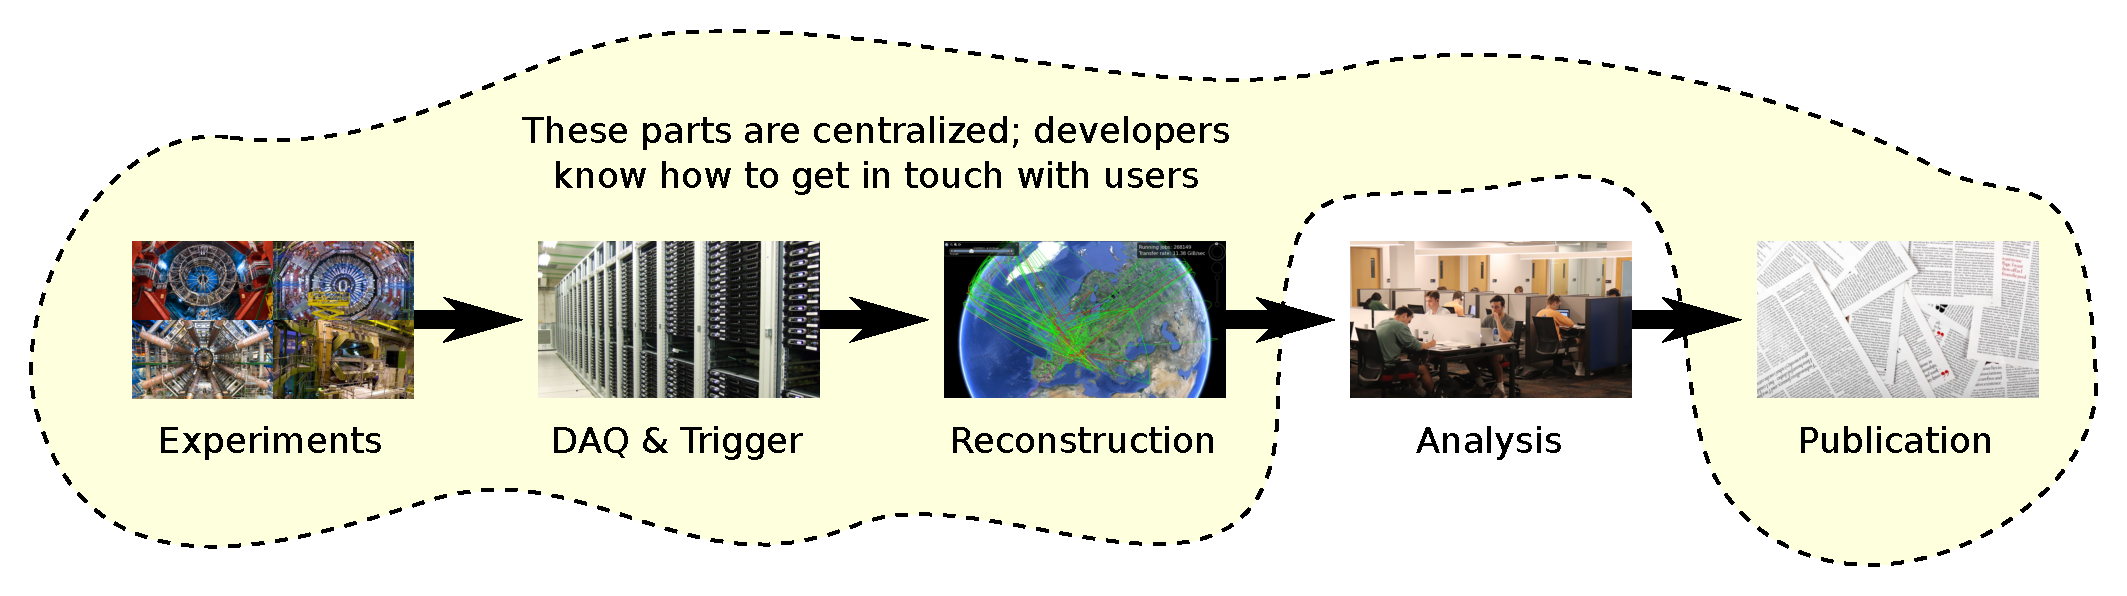
\includegraphics[width=\linewidth]{PLOTS/analysis-chain.pdf}}
\end{columns}

\vspace{0.5 cm}
\begin{itemize}
\item<3-> Good software depends on mutual understanding (between developers and users) of what the software is for and what it can be expected to be able to do.
\item<4-> The ``analysis'' step is the only one in the pipeline for which we don't even know \underline{\it who} all the users are.
\end{itemize}
\end{frame}

\begin{frame}{We don't do this}
\vspace{1 cm}
\begin{center}
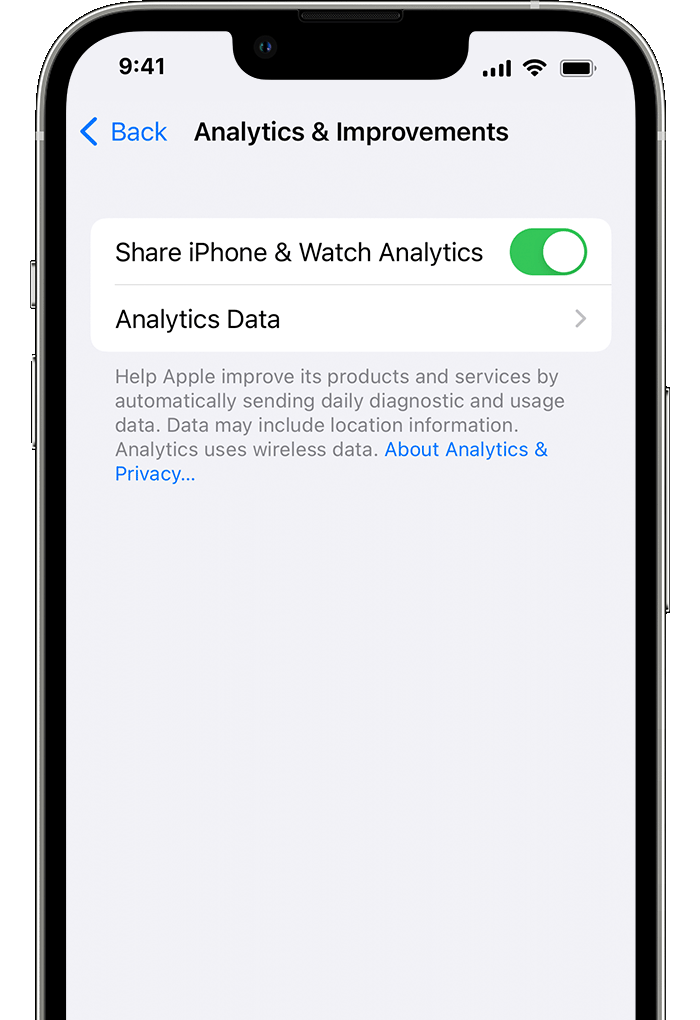
\includegraphics[width=0.5\linewidth]{PLOTS/iphone-send-usage-data.png}
\end{center}
\end{frame}

\begin{frame}{So what can we do instead?}
\vspace{0.35 cm}
\begin{columns}
\column{1.05\linewidth}

\renewcommand{\arraystretch}{0.85}
\begin{tabular}{p{3 cm} p{4.7 cm} p{5.7 cm}}
{\bf Method} & {\bf Good} & {\bf Bad} \\\hline
\uncover<2->{Bug-reports} & \uncover<2->{Resolve immediate needs.} & \uncover<2->{Only hear from proactive people.} \\
\uncover<3->{Surveys} & \uncover<3->{Can directly ask people what they think. Quantitative.} & \uncover<3->{Are the people who didn't fill it out correlated with the questions?} \\
\uncover<4->{Focus groups} & \uncover<4->{As above, but open to free-form, generating new ideas.} & \uncover<4->{Need to follow up from the small group to a large survey.} \\
\uncover<5->{Download stats} & \uncover<5->{People vote with their feet. Quantitative.} & \uncover<5->{Coarse-grained: only know package-level info. Skewed by batch jobs.} \\
\uncover<6->{Textual analysis of CHEP/ACAT} & \uncover<6->{Long-view historical trends.} & \uncover<6->{Only for those who give talks, and what they choose to talk about.} \\
\uncover<7->{\only<1-7>{Analysis of source code online}\only<8>{\textcolor{violet}{Analysis of source code online}}} & \uncover<7->{\only<1-7>{Fine-grained, quantitative, average over many users.}\only<8>{\textcolor{violet}{Fine-grained, quantitative, average over many users.}}} & \uncover<7->{\only<1-7>{Only public repos, have to identify demographics with some seed: how to define ``particle physicists''?}\only<8>{\textcolor{violet}{Only public repos, have to identify demographics with some seed: how to define ``particle physicists''?}}} \\
\end{tabular}
\end{columns}
\end{frame}

\begin{frame}{What download stats are good for (one slide)}
\vspace{0.35 cm}
Relative rates, such as new version adoption.

\begin{center}
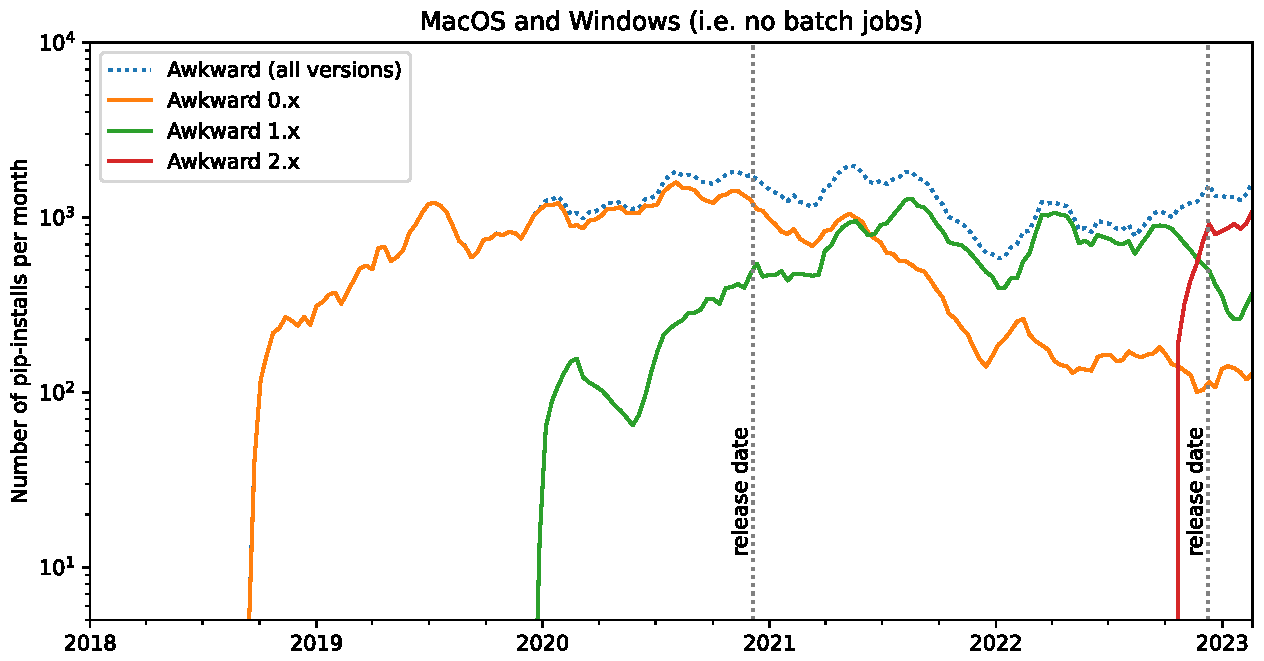
\includegraphics[width=0.9\linewidth]{PLOTS/pip-macwin-awkward-log.pdf}
\end{center}
\end{frame}

\begin{frame}{What textual analysis of CHEP/ACAT is good for (one slide)}
\vspace{0.35 cm}
Discovering trends and changing interests. (``How buzzy is X compared to OOP?'')

\begin{center}
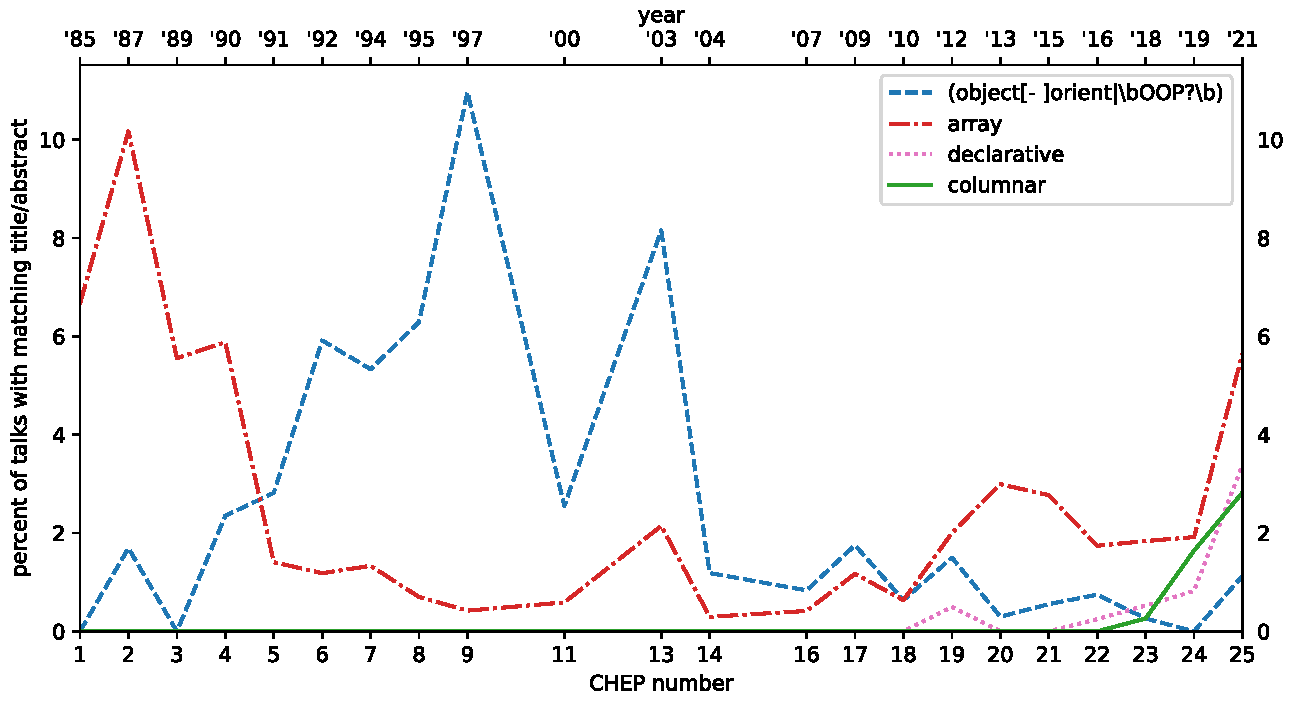
\includegraphics[width=0.9\linewidth]{PLOTS/chep-papers-paradigm.pdf}
\end{center}
\end{frame}

\begin{frame}{Analysis of source code online (the rest of this talk)}
\vspace{0.5 cm}

A few years ago (2019), I stumbled upon a good technique:

\vspace{0.2 cm}
\begin{itemize}
\item CMSSW has been on GitHub since 2013.
\item Many CMS physicists have to fork CMSSW at some point.
\item Very few non-physicists would fork CMSSW.
\end{itemize}

\vspace{0.2 cm}
\uncover<2->{So the technique is: select GitHub users who forked CMSSW (``CMS physicists'') and look at all of their non-fork repos. \textcolor{darkblue}{3\,697 people, 22\,961 repos over 10 years.}}

\vspace{1 cm}
\uncover<3->{\textcolor{darkblue}{But what about experiments other than CMS?}}
\end{frame}

\begin{frame}{A complementary dataset}
\vspace{0.5 cm}
\vspace{\baselineskip}

\begin{itemize}
\item GitHub Archive (\textcolor{blue}{\small\bf\url{https://www.gharchive.org/}}) has been collecting all fork, PR, issue, wiki, watch, and comment events since 2017. We can get a list of GitHub users who have had any interaction at all with a specified repo.
\item \textcolor{blue}{\small\bf\url{https://github.com/root-project/root}} seems like a logical choice to define ``particle physicists.''
\item \textcolor{gray}{(Could also consider a set of repos.)}
\item \textcolor{gray}{(We can get a list of 13\,069 root-forum users, but not their GitHub userids.)}
\end{itemize}

\vspace{0.2 cm}
\uncover<2->{So: select GitHub users who interacted with the ROOT repo (``particle physicists'') and look at all of their non-fork repos. \textcolor{darkblue}{2\,824 people, 17\,334 repos over 6 years.}}

\vspace{0.5 cm}
\uncover<3->{Interestingly, only 143 are in both (3.9\% of CMSSW and 5.1\% of ROOT).}
\end{frame}

\begin{frame}{What they said in their profile bios}
\vspace{0.5 cm}
\begin{columns}
\column{0.55\linewidth}
\mbox{ } \hfill \textcolor{darkblue}{\large Selected by CMSSW fork} \hfill \mbox{ }

\vspace{0.2 cm}
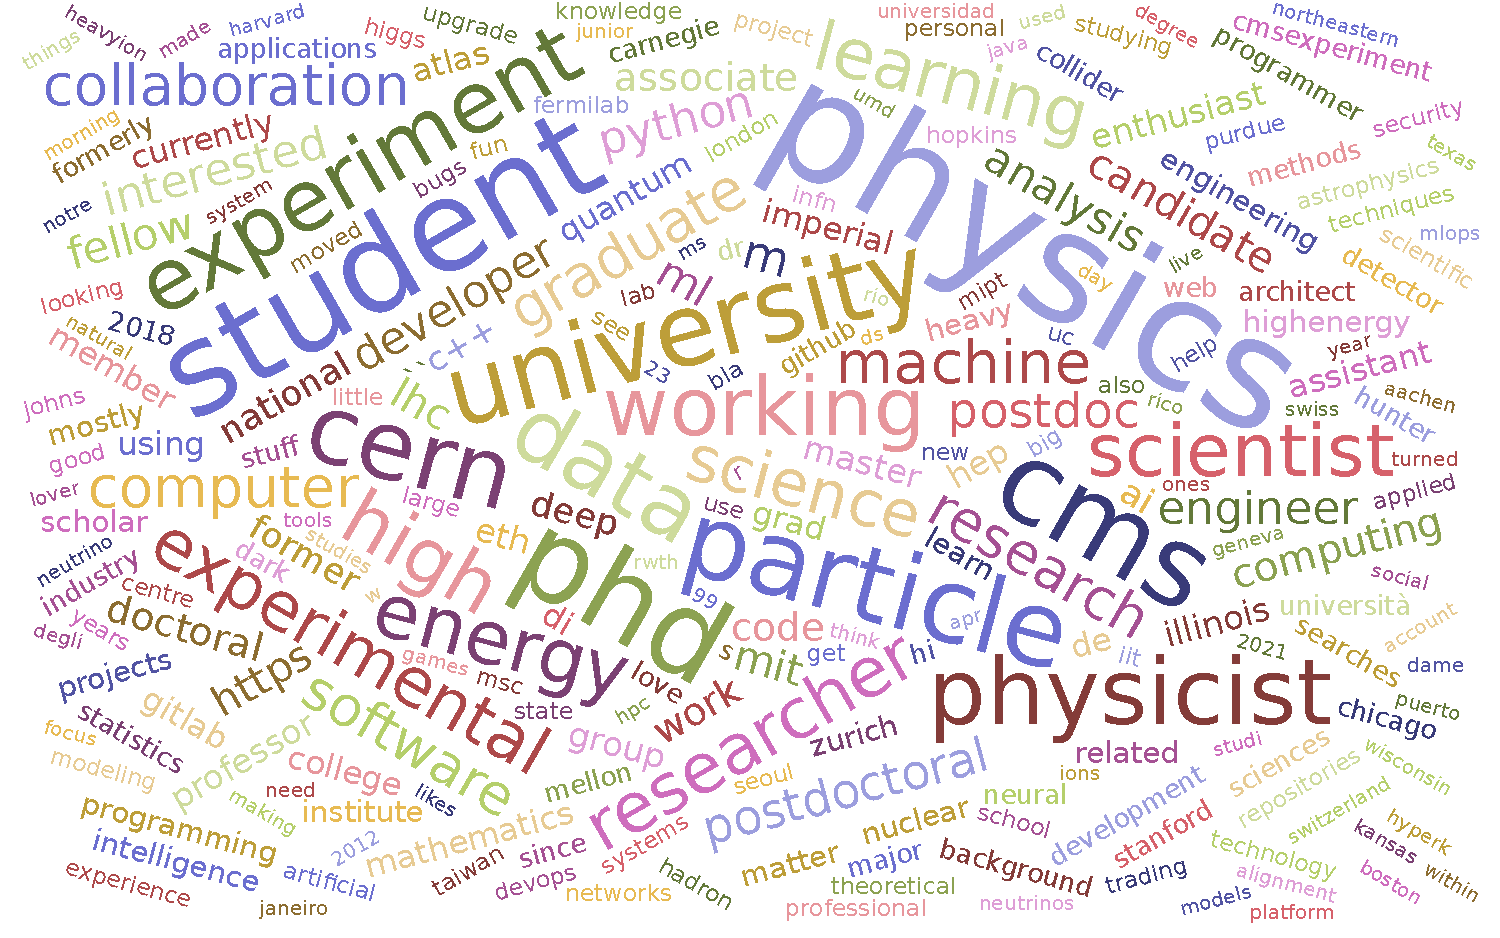
\includegraphics[width=\linewidth]{PLOTS/cmssw-profile-bios-wordcloud.pdf}

\begin{center}
\begin{minipage}{0.9\linewidth}
A lot of ``physics,'' ``student,'' ``particle,'' ``physicist,'' ``PhD,'' ``CERN,'' and ``CMS.''
\end{minipage}
\end{center}

\column{0.55\linewidth}
\mbox{ } \hfill \textcolor{darkblue}{\large Selected by ROOT interaction} \hfill \mbox{ }

\vspace{0.2 cm}
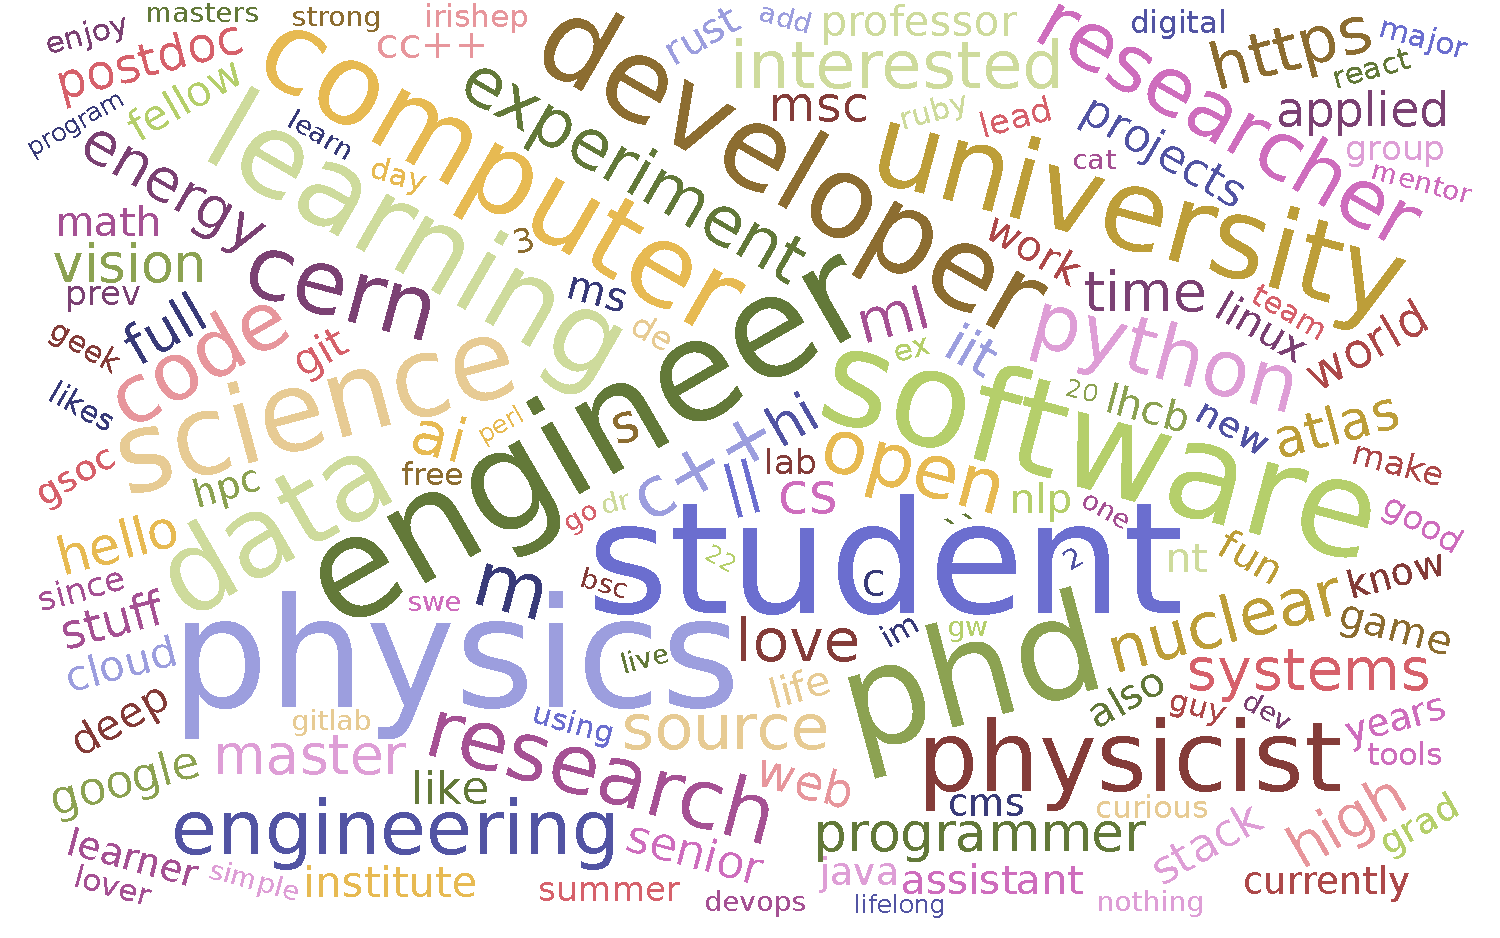
\includegraphics[width=\linewidth]{PLOTS/root-repo-profile-bios-wordcloud.pdf}

\begin{center}
\begin{minipage}{0.95\linewidth}
A little more ``software,'' ``engineer,'' but still lots of ``physics,'' ``student,'' and ``PhD.''
\end{minipage}
\end{center}

\end{columns}
\end{frame}

\begin{frame}{What can we do once we have the repos?}
\vspace{0.5 cm}
Previously, I regex-searched them for ``\mintinline{python}{import XYZ}'' and ``\EscMintinline{c++}{\#include<XYZ>}''.

\vspace{0.5 cm}
\uncover<2->{For this talk, I wanted to go further and build ASTs/statically analyze all of the code.}

\vspace{0.5 cm}
\begin{uncoverenv}<3->
I wasn't first to have this idea: see Chris Ostrouchov's \textcolor{blue}{\href{https://labs.quansight.org/blog/2019/05/python-package-function-usage}{Measuring API Usage}} (2019).

\begin{center}
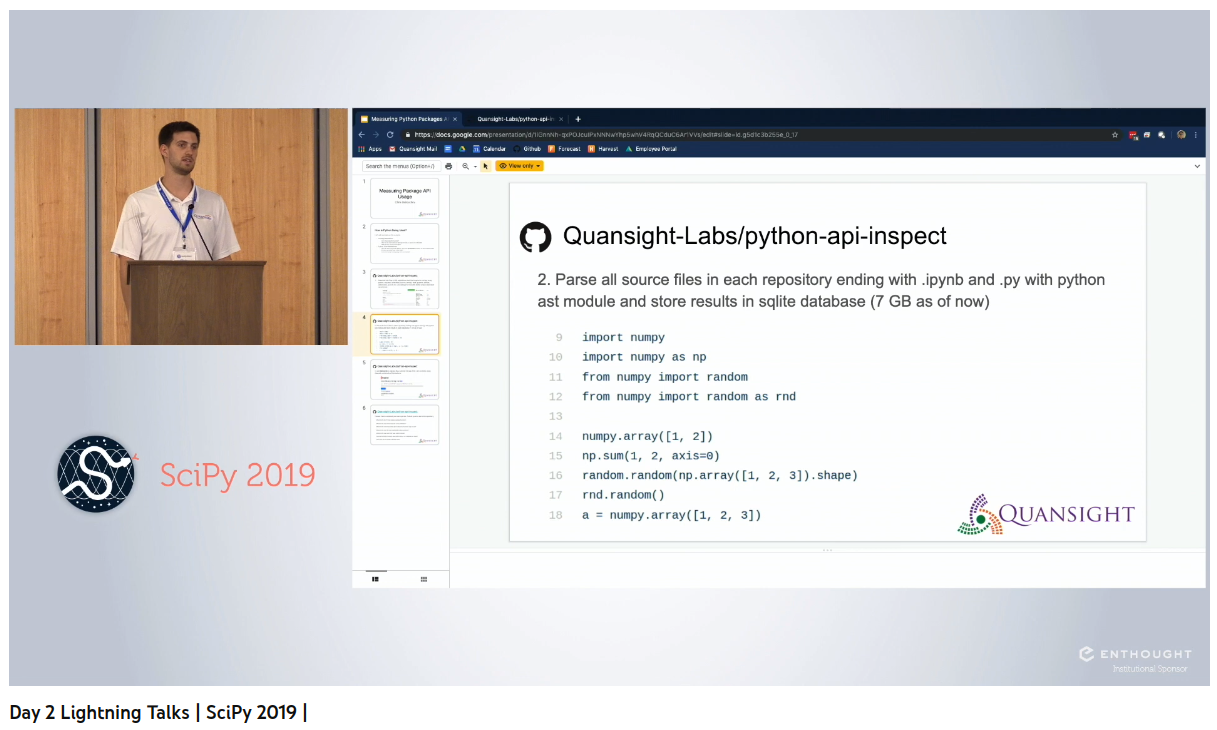
\includegraphics[width=0.55\linewidth]{PLOTS/chris-ostrouchov.png}
\end{center}
\end{uncoverenv}
\end{frame}

\begin{frame}{But first, reproducing the previous studies}
\vspace{0.5 cm}

\textcolor{gray}{Note that the data have changed: more GitHub users have forked CMSSW since the last time we looked, which adds even their past history to the plot, and the date of a repo is set by the latest file, which causes them to migrate bins (forward in time).}

\begin{columns}
\column{0.58\linewidth}
\hspace{-0.4 cm}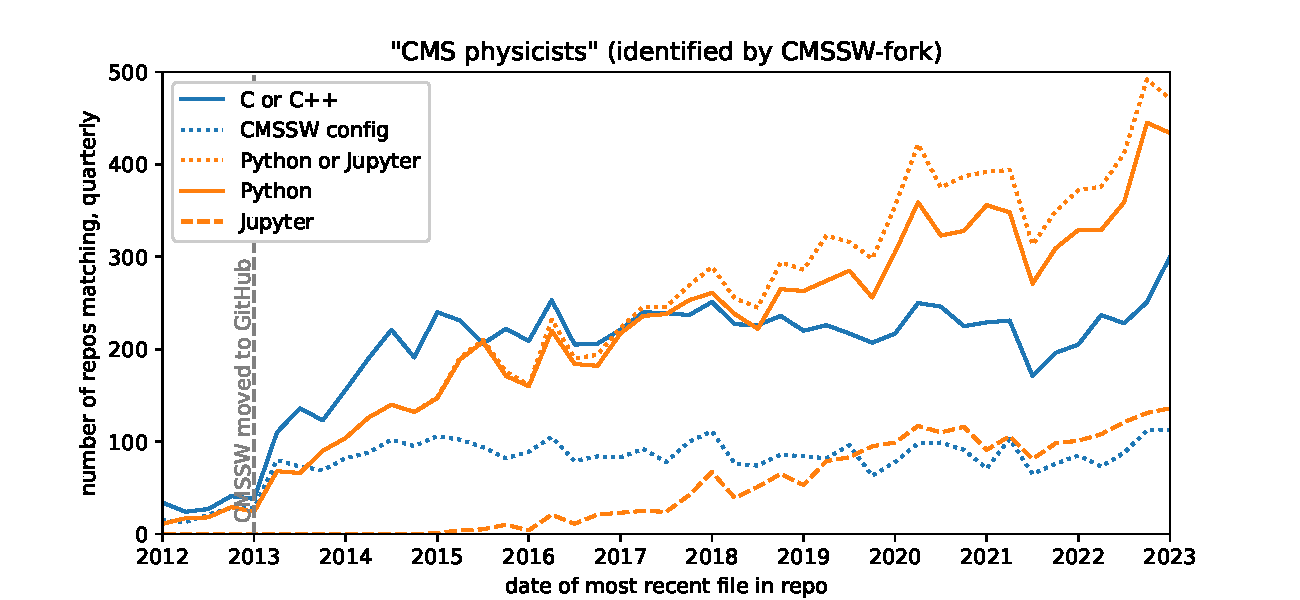
\includegraphics[width=1.05\linewidth]{analysis/github-language-cmsswseed.pdf}

\column{0.58\linewidth}
\hspace{-0.45 cm}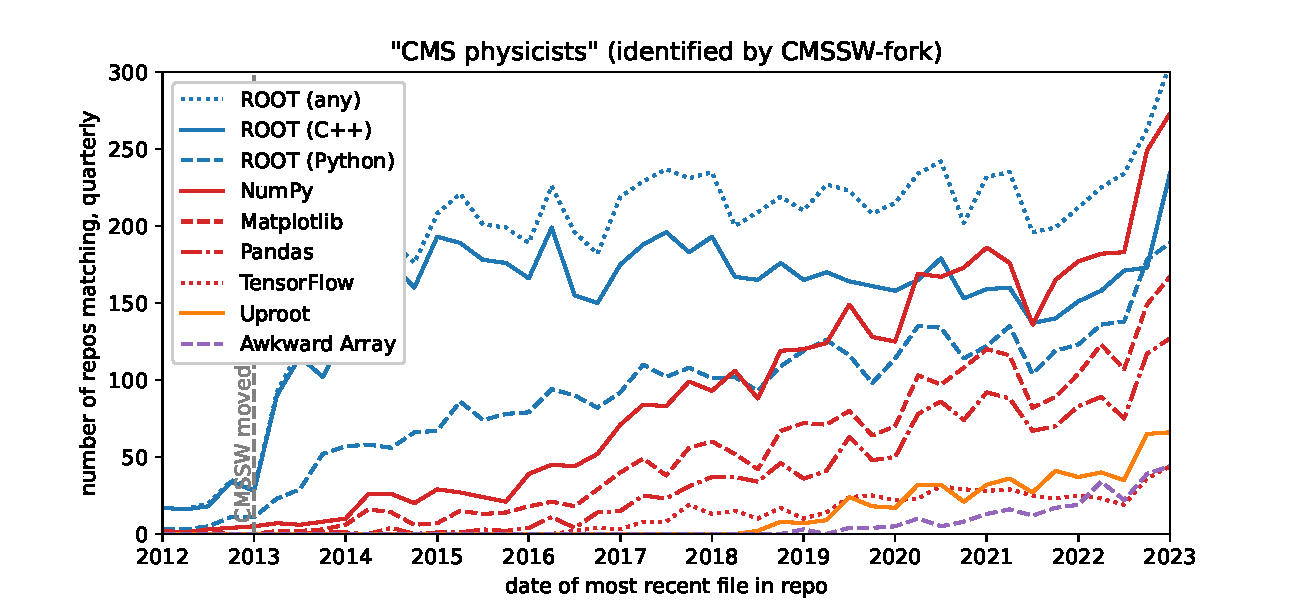
\includegraphics[width=1.05\linewidth]{analysis/github-package-cmsswseed.pdf}
\end{columns}

\begin{columns}
\column{0.5\linewidth}

\small
\uncover<2->{Conclusion is the same: C++ and CMSSW config (Python with \mintinline{python}{import FWCore}) are flat, while Python and Jupyter (Python) increase.}

\column{0.5\linewidth}

\small
\uncover<3->{Conclusion is the same: ROOT-C++ usage is flat while PyROOT and especially NumPy, Matplotlib, Pandas, TensorFlow are increasing. \uncover<4->{Uproot/Awkward usage $\sim$ TensorFlow usage.}}

\end{columns}
\end{frame}

\begin{frame}{Better represented as fractions: \#matching repos/\#total repos}
\begin{columns}
\column{0.6\linewidth}
\hspace{-0.45 cm}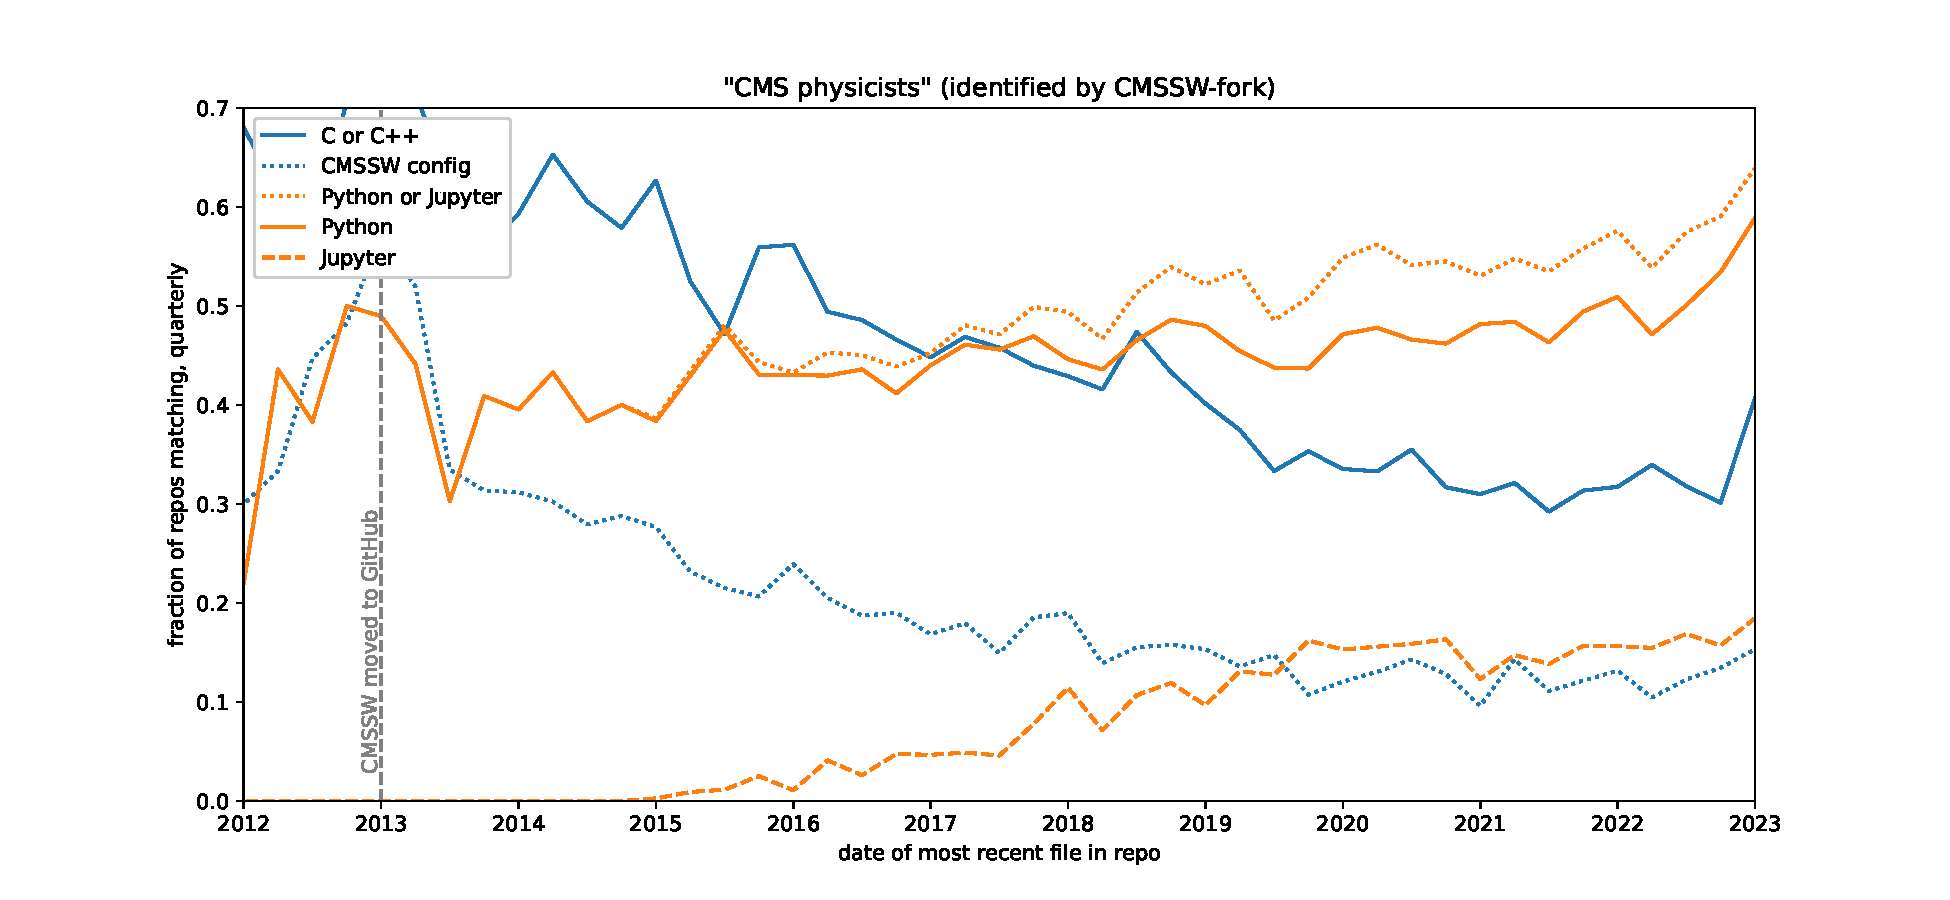
\includegraphics[width=1.05\linewidth]{analysis/github-language-cmsswseed-fraction.pdf}

\column{0.6\linewidth}
\hspace{-0.75 cm}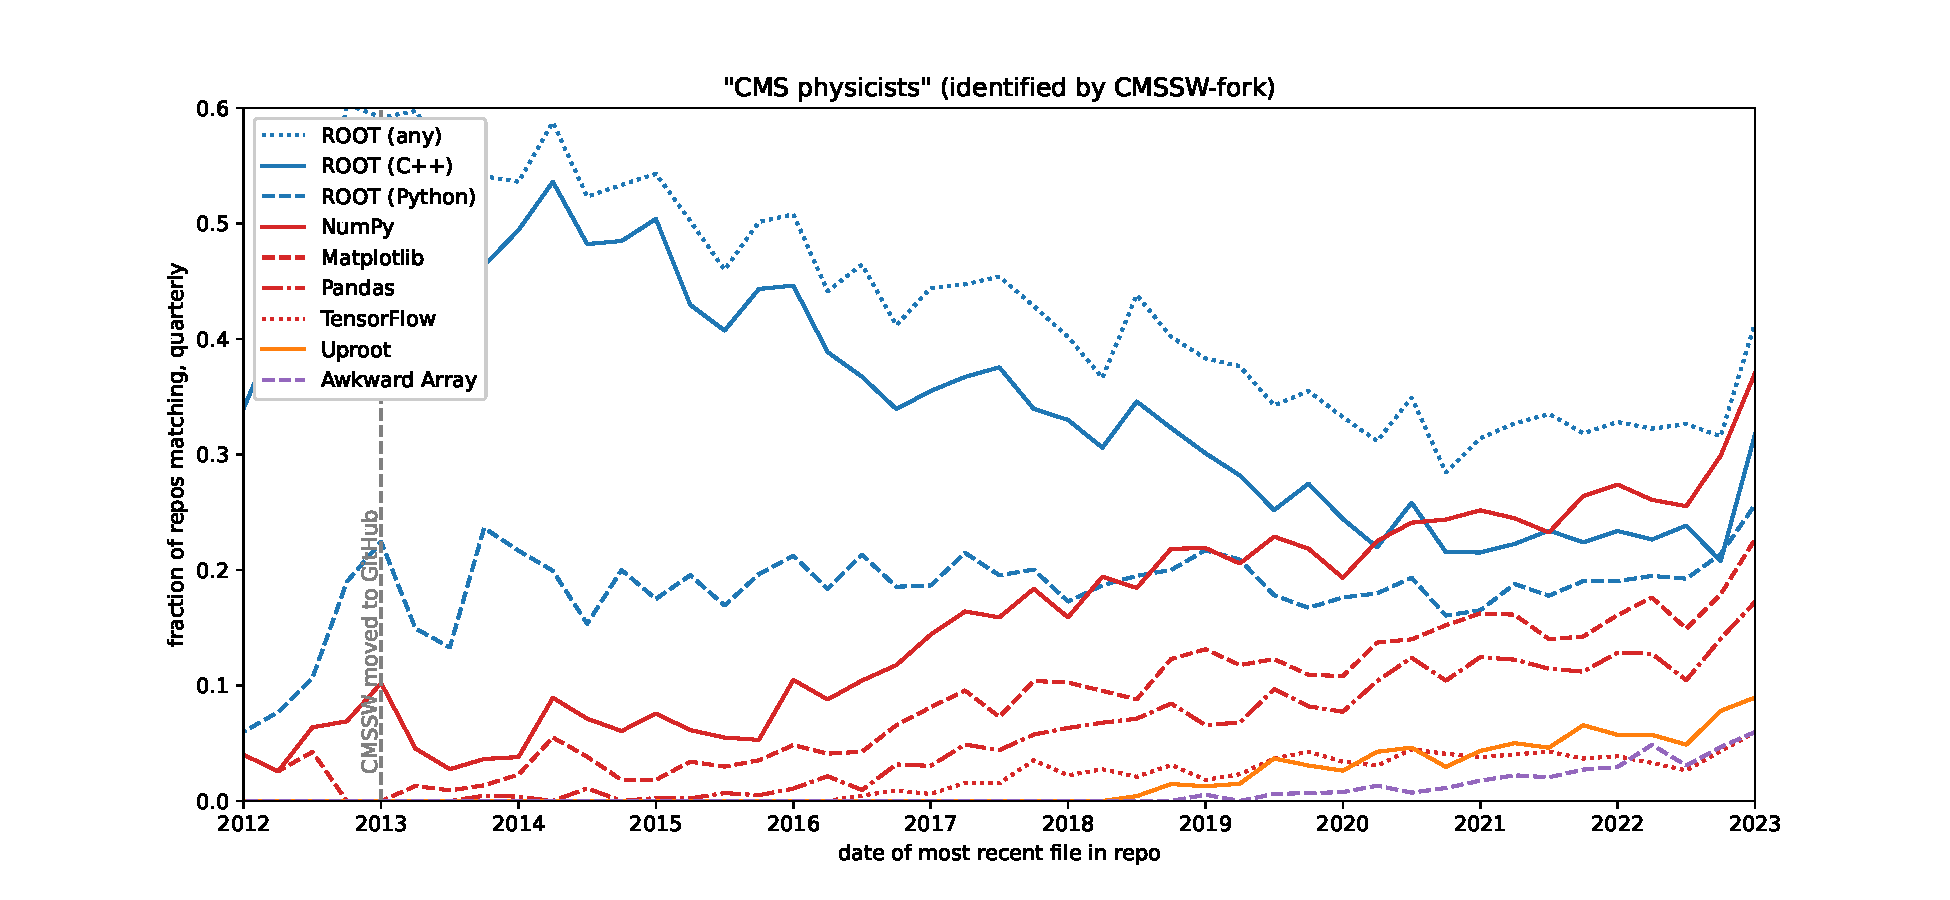
\includegraphics[width=1.05\linewidth]{analysis/github-package-cmsswseed-fraction.pdf}
\end{columns}

\vspace{-0.08 cm}
\begin{columns}
\column{0.6\linewidth}
\uncover<2->{\hspace{-0.45 cm}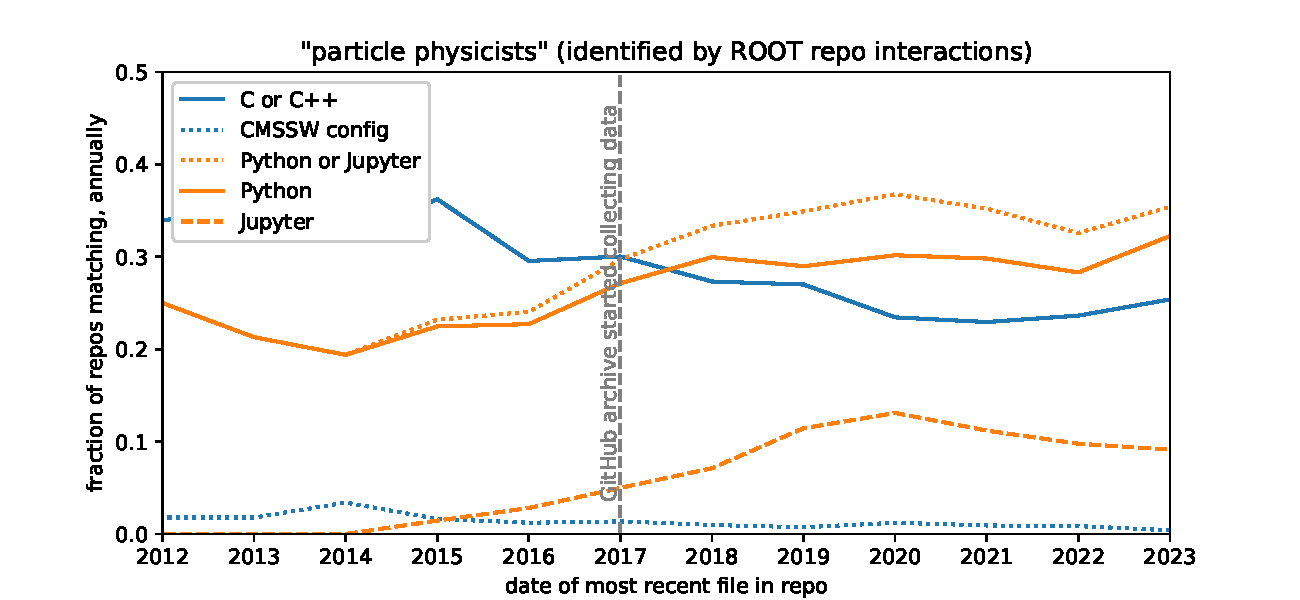
\includegraphics[width=1.05\linewidth]{analysis/github-language-rootseed-fraction.pdf}}

\column{0.6\linewidth}
\uncover<2->{\hspace{-0.75 cm}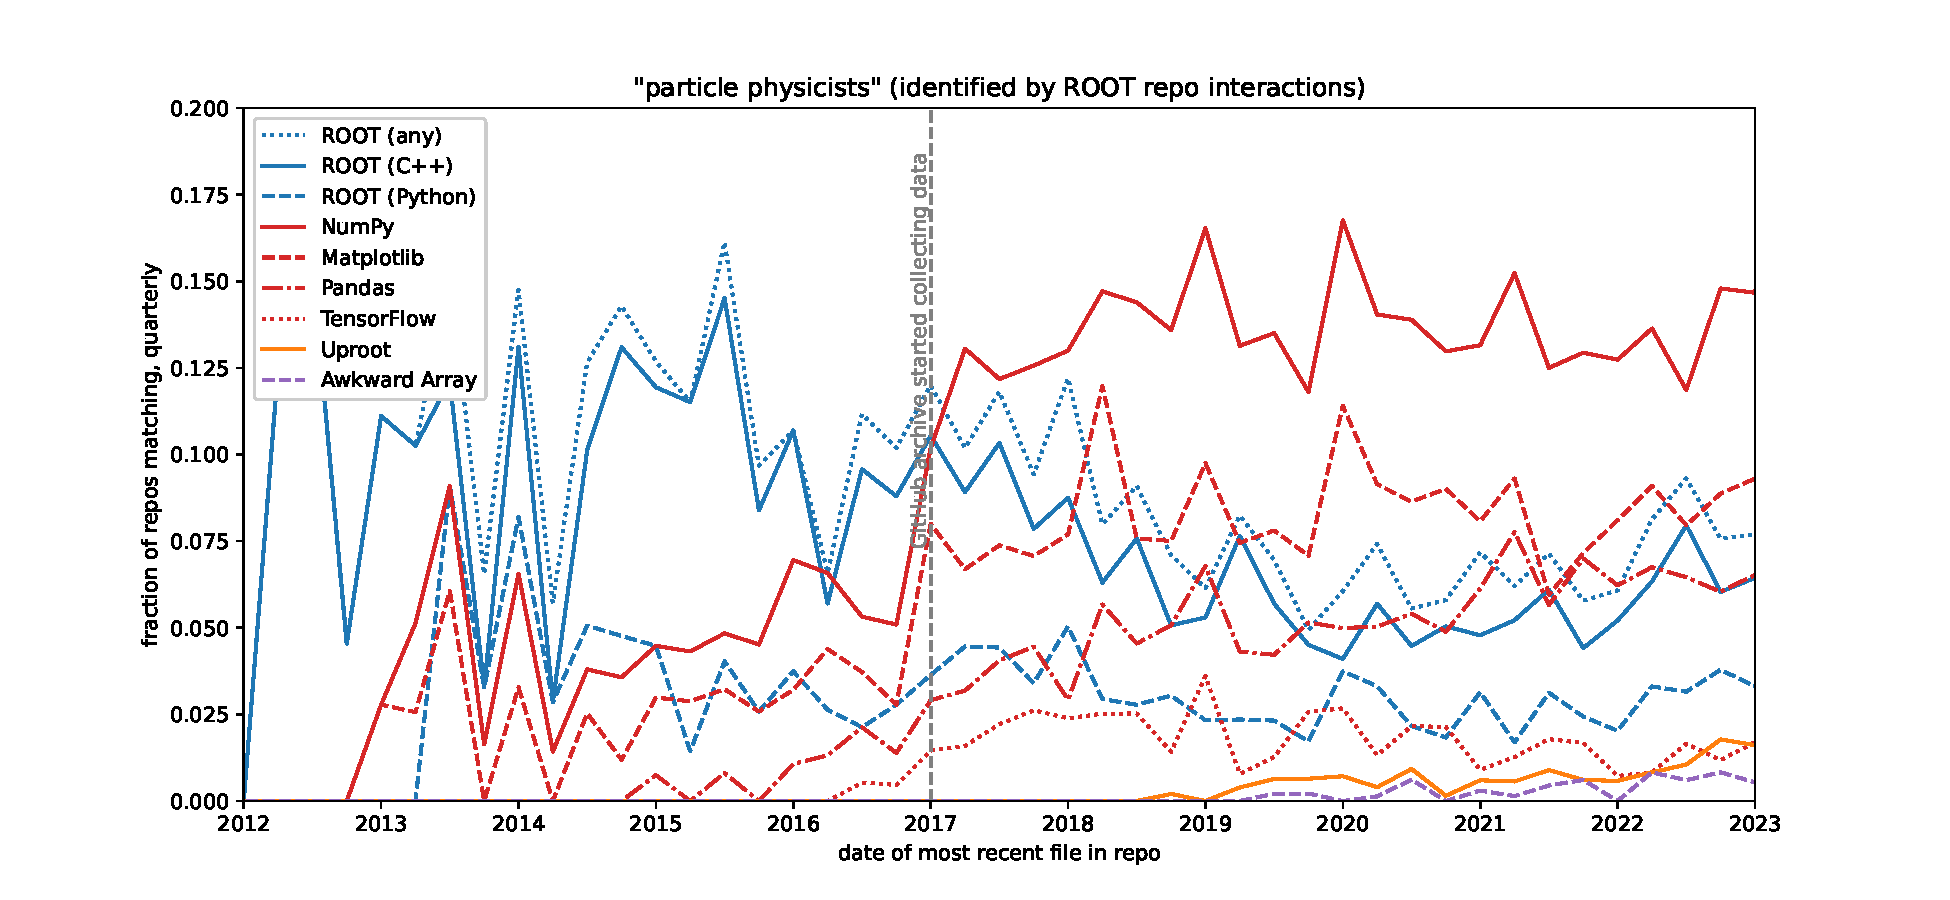
\includegraphics[width=1.05\linewidth]{analysis/github-package-rootseed-fraction.pdf}}
\end{columns}

\begin{uncoverenv}<3->
\vspace{-6.8 cm}
\mbox{ } \hfill \fcolorbox{darkblue}{white}{\begin{minipage}{0.5\linewidth}
\textcolor{darkblue}{Some of the growth was in the denominator: the total number of repos is increasing while Python use also increases.}
\end{minipage}} \hfill \mbox{ }
\vspace{6.8 cm}
\end{uncoverenv}

\begin{uncoverenv}<4->
\vspace{-4.6 cm}
\mbox{ } \hfill \fcolorbox{darkblue}{white}{\begin{minipage}{0.5\linewidth}
\textcolor{darkblue}{In the ROOT-selected group, Python use has always been higher, though the profile bios indicated more engineers and computer scientists.}
\end{minipage}} \hfill \mbox{ }
\vspace{4.6 cm}
\end{uncoverenv}
\end{frame}

\begin{frame}{Can we select physicists using their profile bios?}
\vspace{0.15 cm}
\small
\begin{columns}
\column{1.07\linewidth}
Regex \mintinline{python}{(phys|analy|hep|particle|cern|cms|atlas|alice|lhc)} selects \textcolor{darkblue}{7.6\% of users}.
\end{columns}

\begin{columns}
\column{0.58\linewidth}
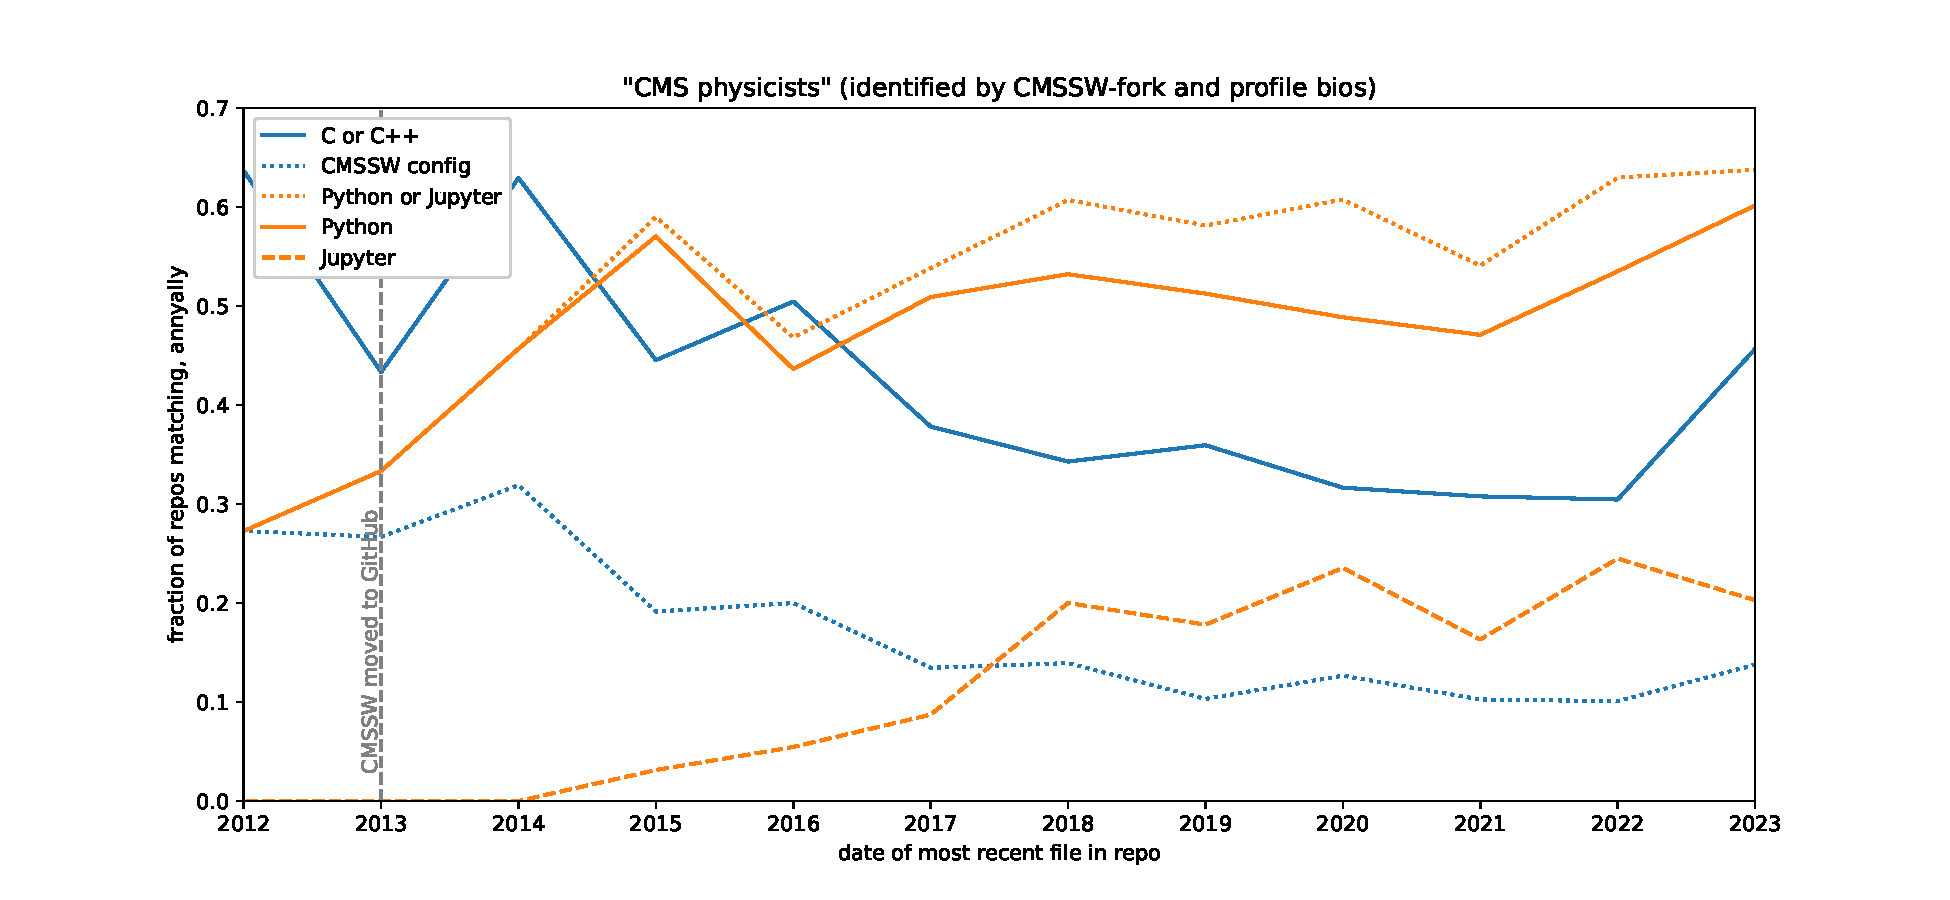
\includegraphics[width=\linewidth]{analysis/github-language-cmsswseed-tight-fraction.pdf}

\column{0.58\linewidth}
\hspace{-0.25 cm}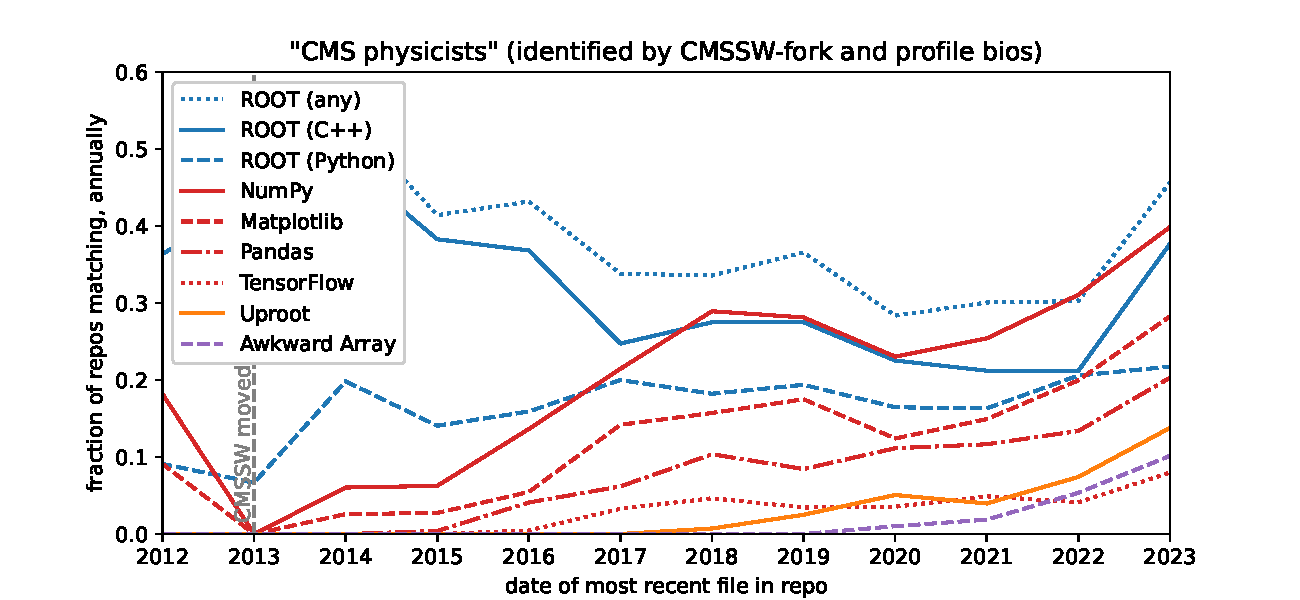
\includegraphics[width=\linewidth]{analysis/github-package-cmsswseed-tight-fraction.pdf}
\end{columns}

\vspace{-0.25 cm}
\begin{columns}
\column{0.58\linewidth}
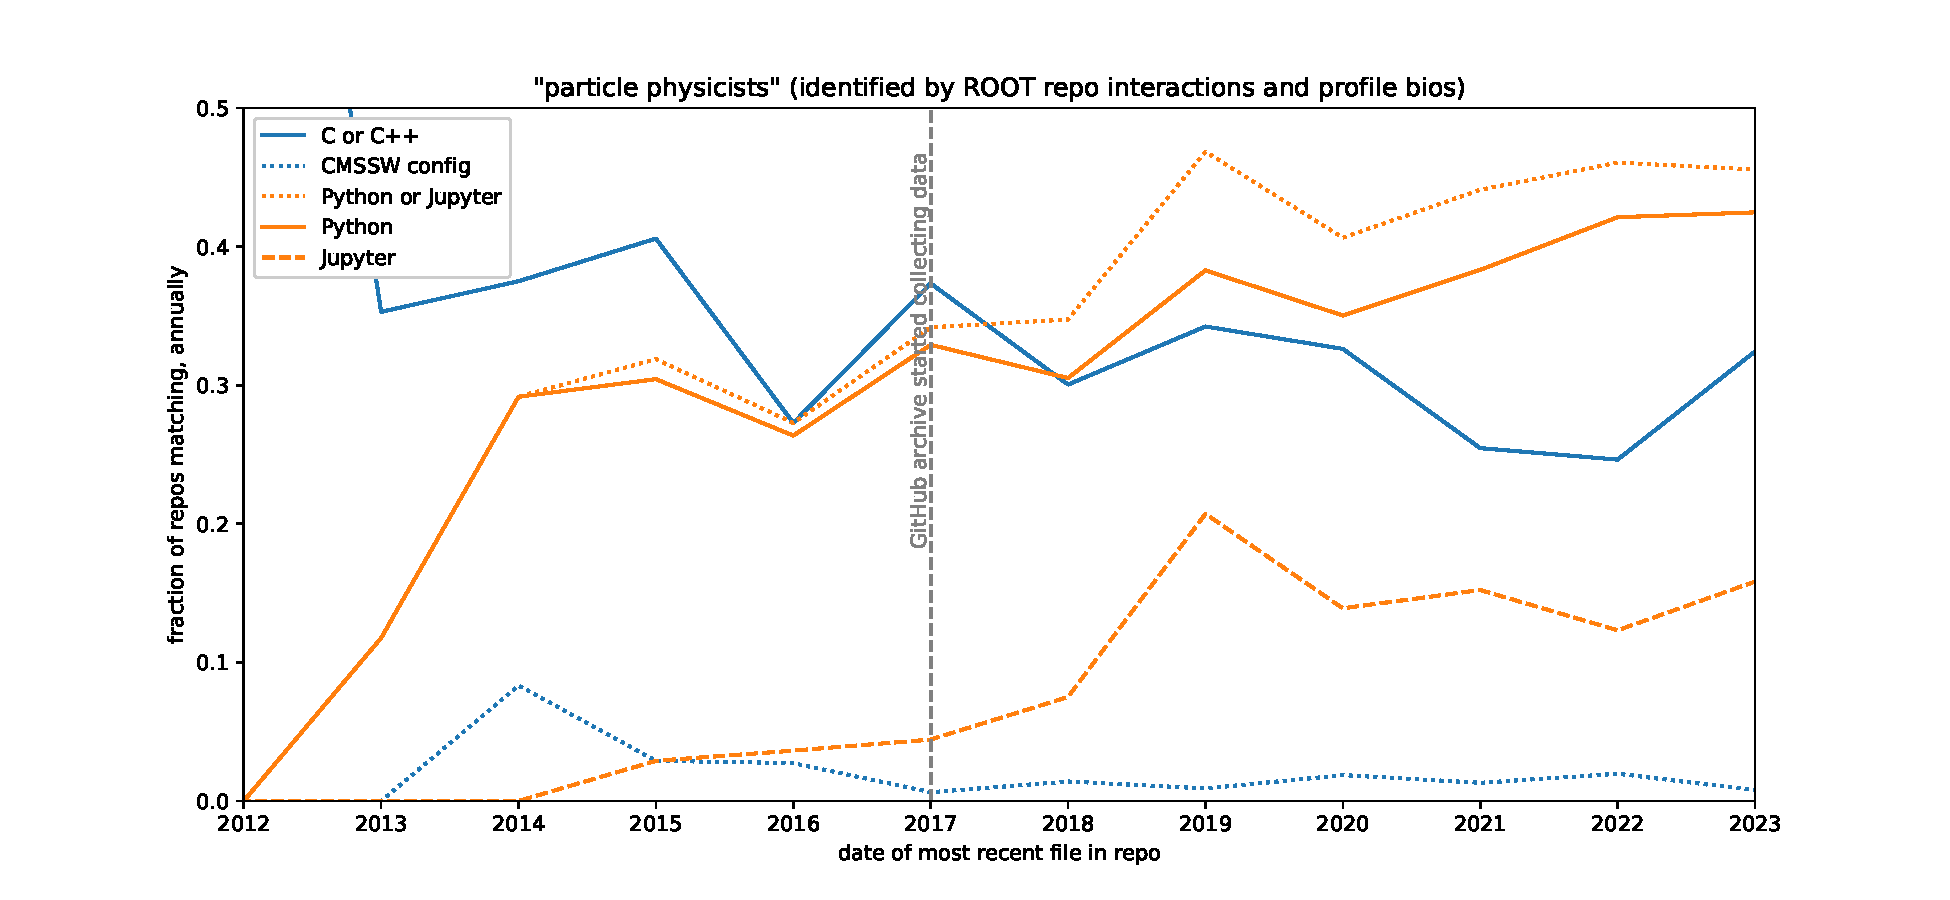
\includegraphics[width=\linewidth]{analysis/github-language-rootseed-tight-fraction.pdf}

\column{0.58\linewidth}
\hspace{-0.25 cm}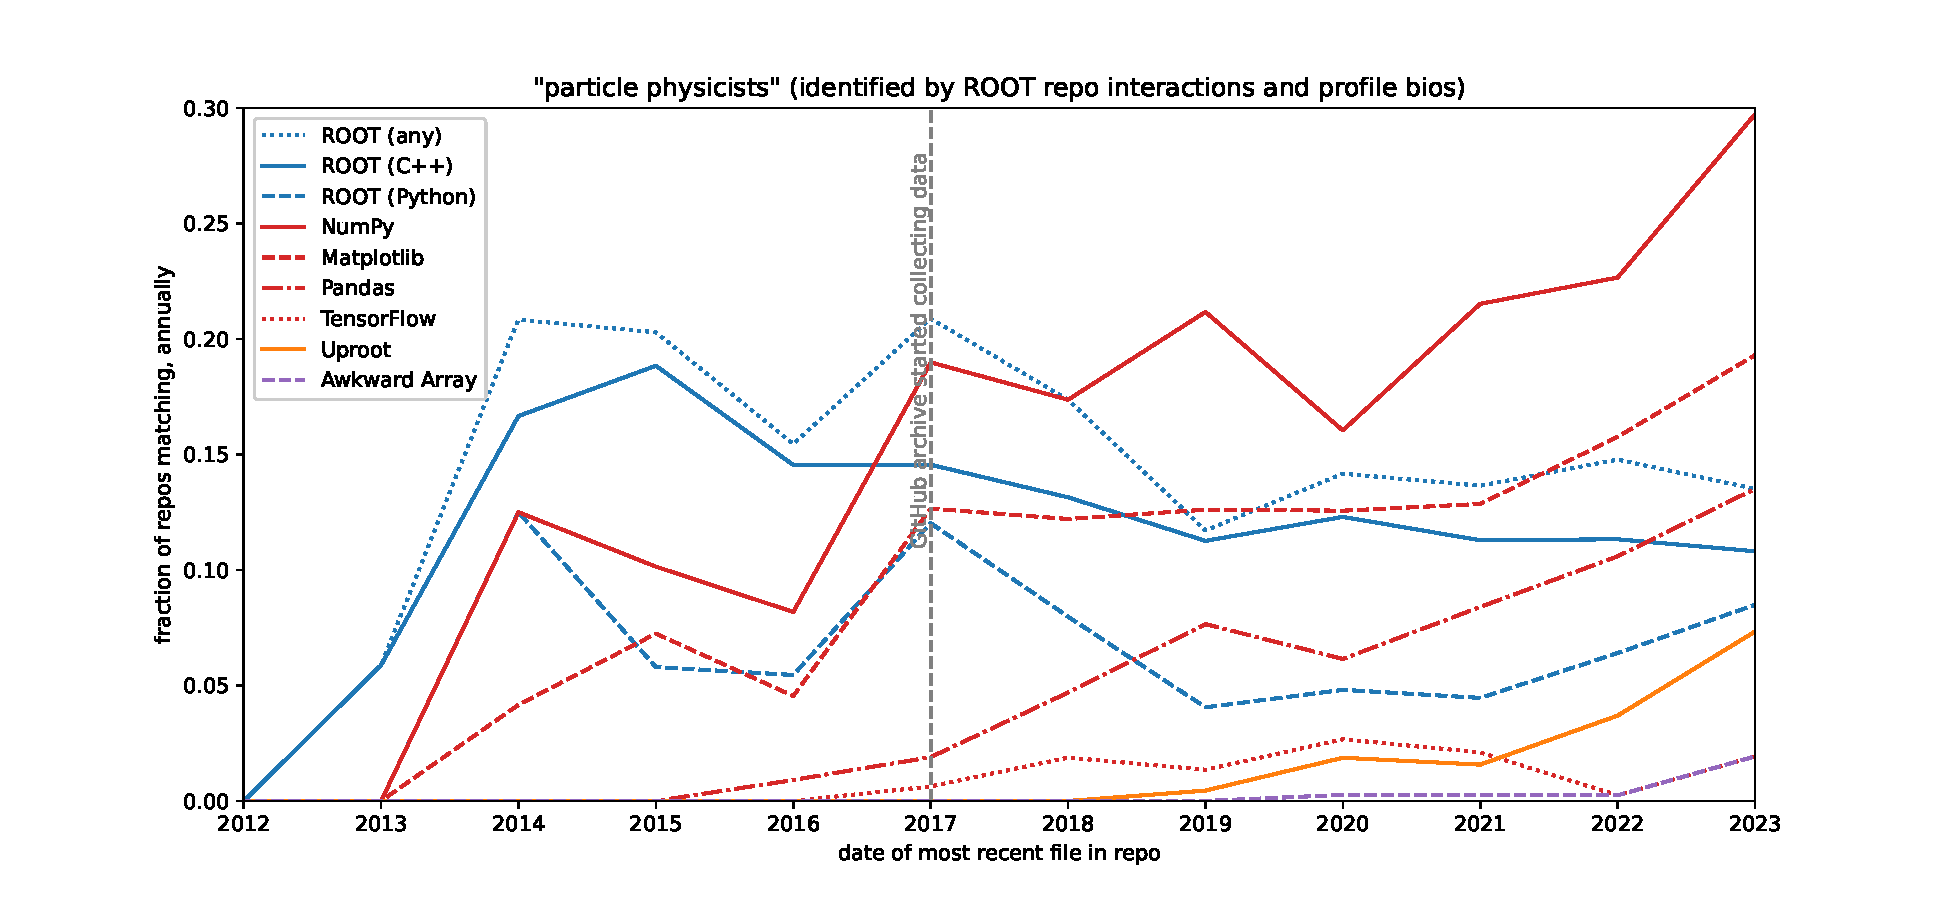
\includegraphics[width=\linewidth]{analysis/github-package-rootseed-tight-fraction.pdf}
\end{columns}

\begin{uncoverenv}<2->
\vspace{-4.3 cm}
\mbox{ } \hfill \fcolorbox{darkblue}{white}{\begin{minipage}{0.5\linewidth}
\textcolor{darkblue}{Although selecting a pure sample of physicists cuts more than 90\% of the data, the same trends are still visible.}
\end{minipage}} \hfill \mbox{ }
\vspace{4.3 cm}
\end{uncoverenv}
\end{frame}

\begin{frame}{Now actually parse the repos: Python 3 adoption among physicists}
\begin{columns}
\column{1.15\linewidth}
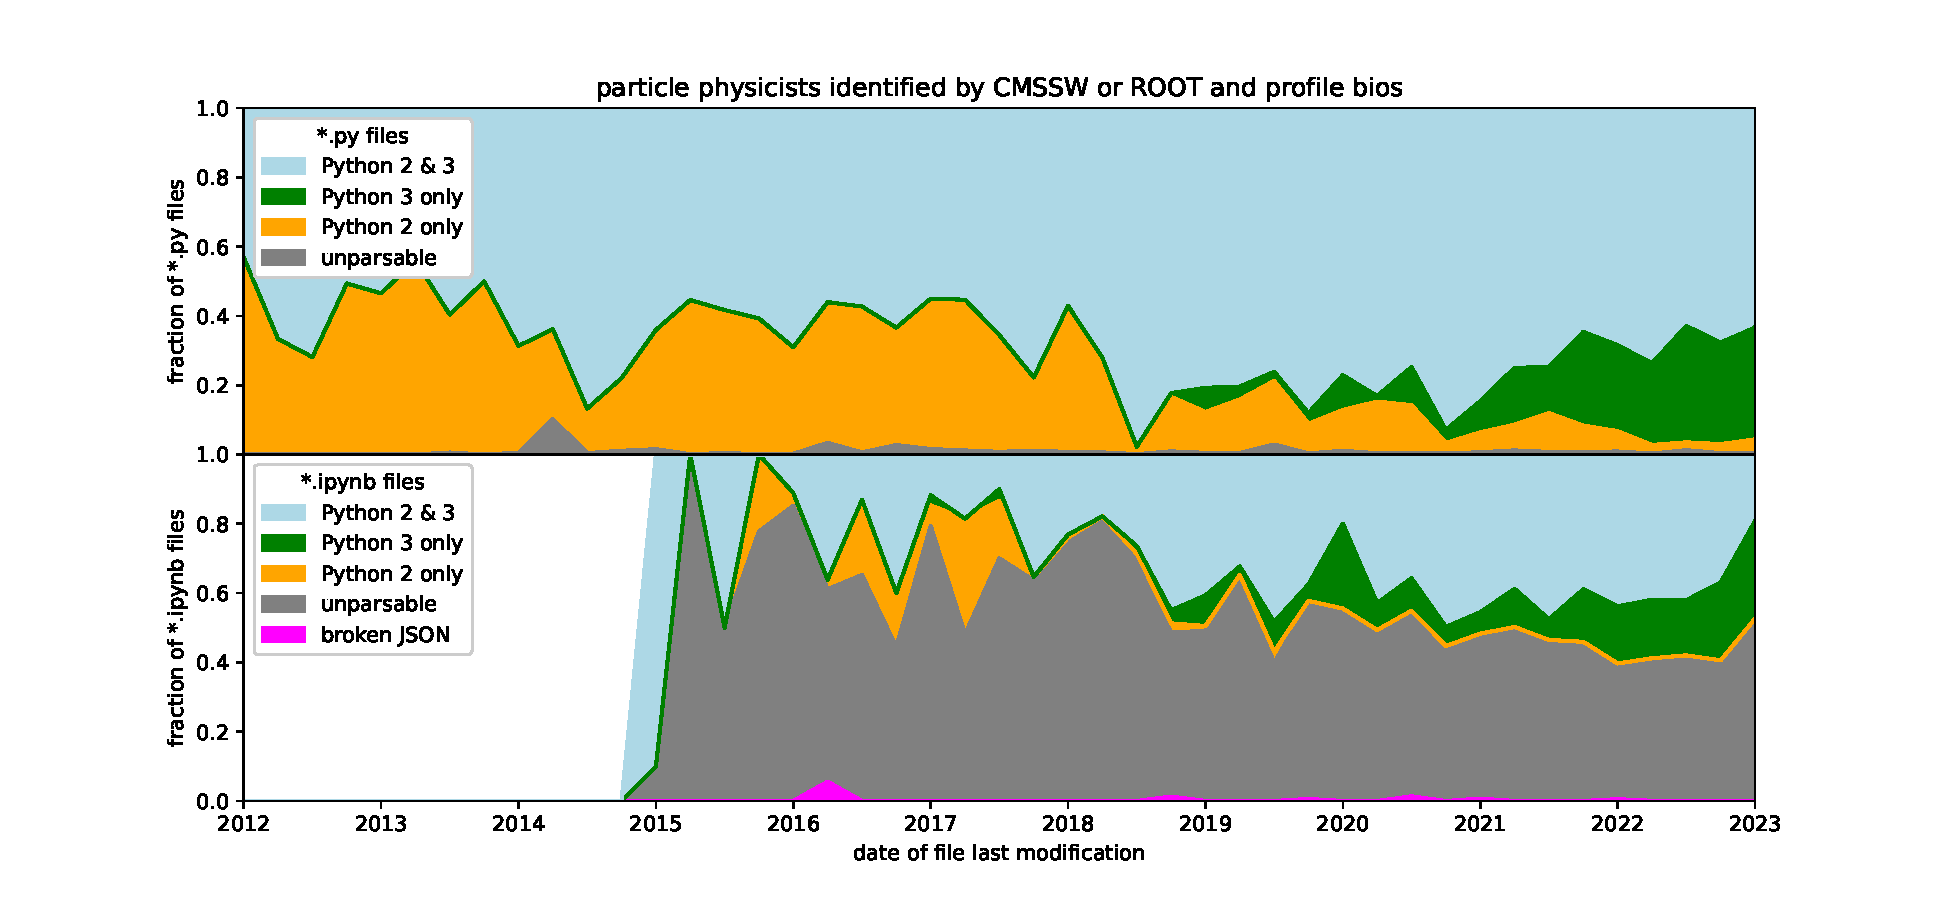
\includegraphics[width=\linewidth]{analysis/github-python-2-3-fraction.pdf}
\end{columns}
\end{frame}

\begin{frame}[fragile]{Ask specific questions: Awkward 1 adoption by function name}
\vspace{0.15 cm}
\begin{columns}
\column{0.7\linewidth}
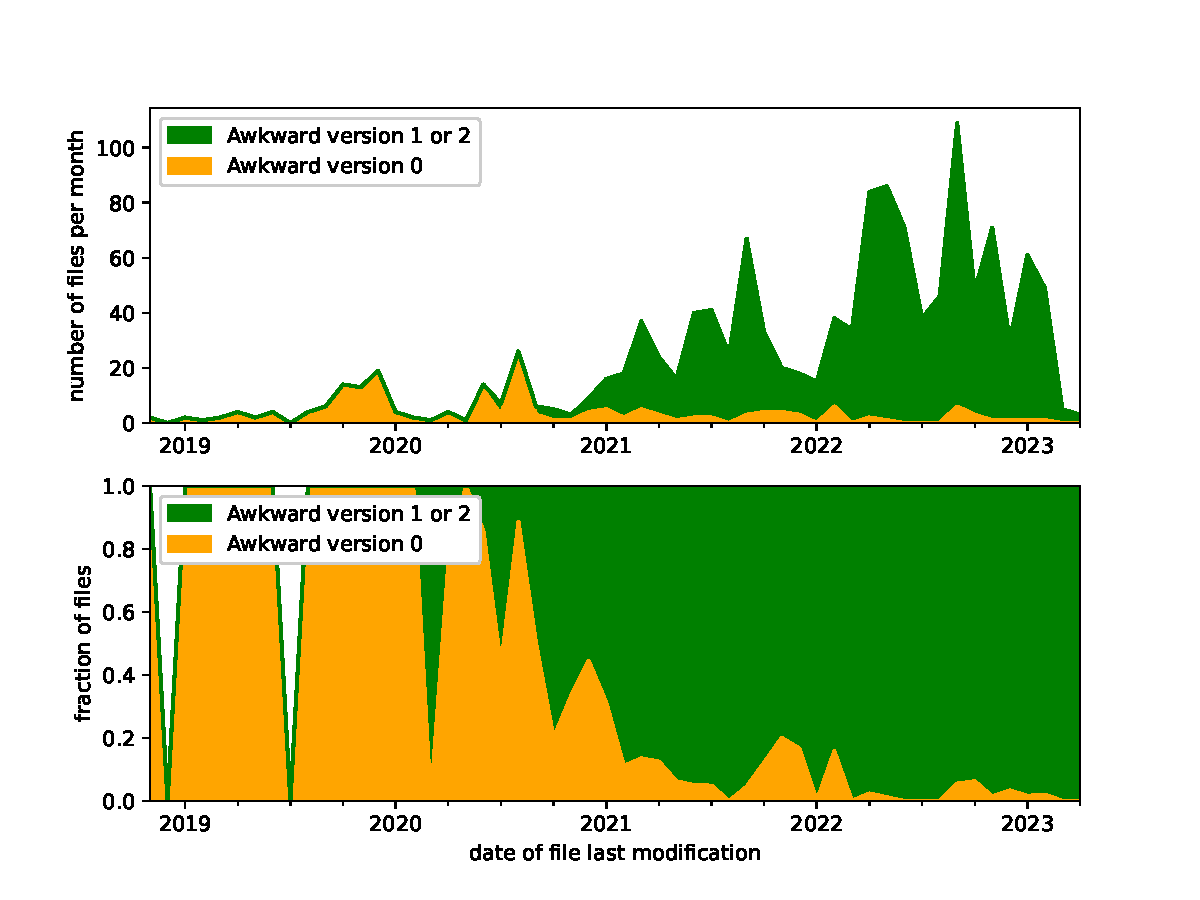
\includegraphics[width=\linewidth]{analysis/github-ast-awkward-0-1.pdf}

\column{0.5\linewidth}
\hspace{-0.7 cm}\begin{minipage}{\linewidth}
\scriptsize
\begin{minted}{python}
def is_awkward0(obj):
    return obj.function.name.startswith(
        "ak.JaggedArray"
    ) or obj.function.name.startswith(
        "ak.array.jagged.JaggedArray"
    ) or obj.function.name in (
            "ak.IndexedArray",
            "ak.Table",
            "ak.fromarrow",
            "ak.fromiter",
            "ak.hdf5",
            "ak.load",
            "ak.save",
            "ak.toarrow",
            "ak.topandas",
            "ak.util.concatenate",
        )
\end{minted}
\end{minipage}
\end{columns}
\end{frame}

\begin{frame}[fragile]{Most common function calls/argument patterns}
\vspace{0.25 cm}
\small
\begin{columns}
\column{0.45\linewidth}
\mbox{\hspace{1.35 cm}{\large\bf Awkward Array}}

\vspace{0.05 cm}
\begin{tabular}{r l}
2832 & \verb|ak.flatten(?)| \\
2498 & \verb|ak.num(?)| \\
2193 & \verb|ak.to_numpy(?)| \\
 874 & \verb|ak.sum(?, axis=1)| \\
 865 & \verb|ak.flatten(?, axis=None)| \\
 564 & \verb|ak.sum(?)| \\
 455 & \verb|ak.ones_like(?)| \\
 406 & \verb|ak.Array(?)| \\
 283 & \verb|ak.concatenate(?)| \\
 265 & \verb|ak.singletons(?)| \\
 248 & \verb|ak.num(?, axis=1)| \\
 246 & \verb|ak.concatenate(?, axis=1)| \\
 235 & \verb|ak.any(?, axis=1)| \\
 234 & \verb|ak.zip(?, with_name='str')| \\
 233 & \verb|ak.to_pandas(?)| \\
 226 & \verb|ak.unzip(?)| \\
 221 & \verb|ak.firsts(?)| \\
\end{tabular}

\column{0.65\linewidth}
\mbox{\hspace{1.35 cm}{\large\bf Uproot}}

\vspace{0.05 cm}
\begin{tabular}{r l}
2150 & \verb|uproot.open(?)| \\
 889 & \verb|uproot.open('str')| \\
 198 & \verb|uproot.recreate(?)| \\
 179 & \verb|uproot.tree.TBranchMethods.array(?)| \\
  74 & \verb|uproot.lazy(?)| \\
  58 & \verb|uproot.newtree(?)| \\
  57 & \verb|uproot.pandas.iterate(?, 'str', ['strings'])| \\
  44 & \verb|uproot.open(?, xrootdsource=?)| \\
  23 & \verb|uproot.lazy(?, filter_name=?)| \\
  22 & \verb|uproot.recreate('str')| \\
  18 & \verb|uproot.create(?)| \\
  15 & \verb|uproot.recreate(?, compression=?)| \\
  13 & \verb|uproot.newbranch(?, size='str')| \\
  11 & \verb|uproot.numentries(?, ?)| \\
  11 & \verb|uproot.ArrayCache('str')| \\
  10 & \verb|uproot.numentries(?, ?, total=False)| \\
  10 & \verb|uproot.numentries(?, ?, executor=?, total=False)| \\
\end{tabular}
\end{columns}

\vspace{-5 cm}
\begin{uncoverenv}<2->
\begin{columns}
\column{1.2\linewidth}
\hspace{8.3 cm}\fcolorbox{darkblue}{white}{\begin{minipage}{0.4\linewidth}
\textcolor{darkblue}{Uproot relies more on object methods. We'd have to statically analyze {\it object types}, not functions on global modules, which is hard in a dynamically typed language.}
\end{minipage}}
\end{columns}
\end{uncoverenv}
\vspace{5 cm}
\end{frame}

\begin{frame}{Use feature adoption to make decisions about deprecation}
\vspace{0.75 cm}
\begin{columns}
\column{1.1\linewidth}
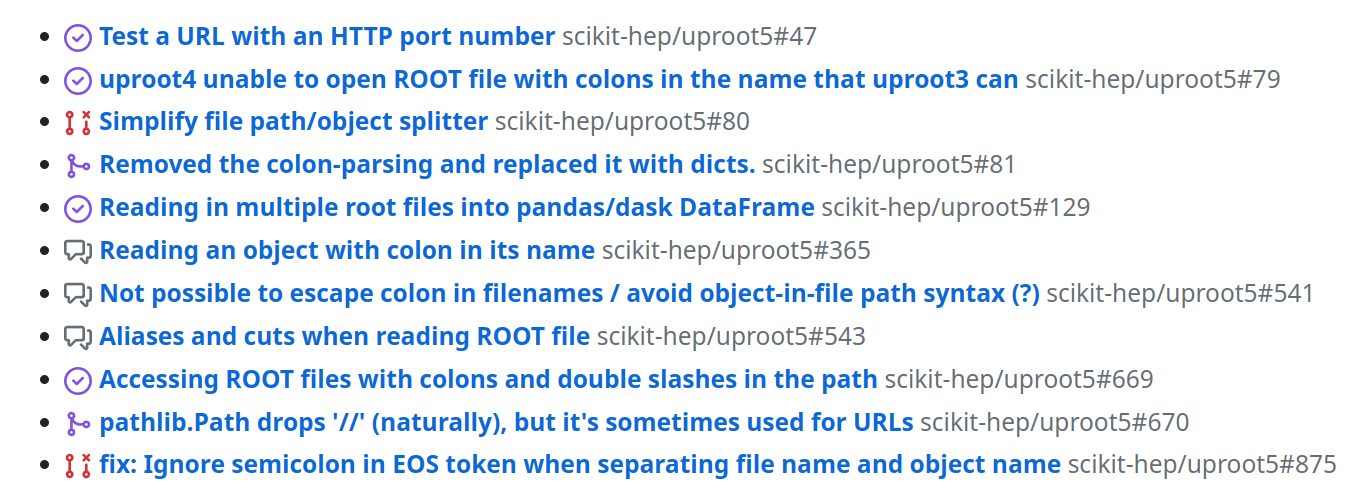
\includegraphics[width=\linewidth]{PLOTS/uproot-open-colon-issues.png}
\end{columns}

\begin{uncoverenv}<2->
\vspace{-6 cm}
\mbox{ } \hfill \fcolorbox{black}{white}{\begin{minipage}{0.65\linewidth}
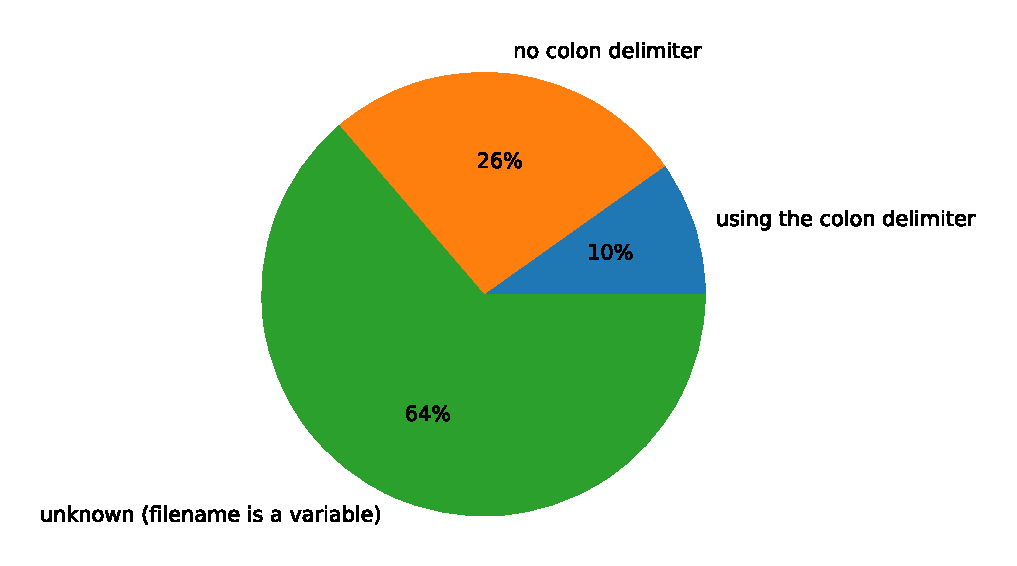
\includegraphics[width=\linewidth]{analysis/github-ast-uproot-filename-colon.pdf}

\mbox{ } \hfill \begin{minipage}{0.75\linewidth}
Removing it would upset many workflows.

The deprecation period has to be {\it long}.
\end{minipage} \hfill \mbox{ }
\end{minipage}} \hfill \mbox{ }
\vspace{6 cm}
\end{uncoverenv}

\end{frame}

\end{document}

